\section{Introduction}
The last several years have seen the emergence of programmable network devices
including both programmable switching chips and programmable network interface
cards (NICs). Along with the rise of x86-based packet processing for
middleboxes and virtual switches, these trends point towards a future where the
entire network will be programmable. The benefits of network programmability
range from commercial use cases such as network virtualization implemented on
the programmable Open vSwitch platform to more recent research projects that
implement packet scheduling, measurement, and application offload of niche
applications on programmable switches.

While the benefits of programmability are clear, they are difficult to reap
because programming the network as a whole remains challenging. Current
programming languages target individual network devices, e.g., P4 for the
Tofino programmable switching chip and the Netronome programmable NIC. However,
at present, there is no unified programming model to express and implement
general data plane functionality at the level of an entire network, without
having to individually program each network device.

Prior work has looked at the problem of programming at the level of an entire
network. In particular, Maple~\cite{maple} was an early example of a
network-wide programming model designed for OpenFlow switches. Maple
automatically divided functionality between a stateless component running on
switches and a stateful component running on the network's controller.
SNAP~\cite{snap} is a more recent example of network-wide programming; unlike
Maple, it additionally offloads stateful functionality to switches by
leveraging stateful processing available in programmable switches.  However,
both Maple and SNAP cannot express programmable-switch functionality that
affects network performance at fine time scales, e.g., packet scheduling,
congestion control, fine-grained measurement of microbursts, and load
balancing. In other words, Maple and SNAP generate highly optimized code, but
are restricted in what they can express.

This demo presents \textbf{Sluice}, a programming model that takes a
network-wide specification of the data plane and compiles it into runnable code
that can be launched directly on the programmable devices of a network. In
contrast to prior network-wide programming models like SNAP and Maple that were
focused on specific tasks (e.g., routing and security policies), Sluice aims to
be more general, but potentially at the cost of quality of generated code.
Sluice endows network operators with the ability to design and deploy large
network programs for various functions such as scheduling, measurement, and
application offloading.  The benefits of Sluice can be summarized as follows: (1) Sluice provides the same functionality as a per-device language like P4 but makes it easier to program the data plane of an entire network by abstracting device-specific architectural details like stateful ALUs, pipelines, etc., and (2) Sluice automatically reduces the amount of boilerplate code needed to write data plane functionality. For instance, the 8 line traffic matrix Sluice program we demonstrate translates into over 200 lines of P4 code. We demonstrate Sluice's functionality and ease of use via two examples: traffic matrix generation for network analysis and a streaming join-filter operation.
\begin{figure}[tp]
\centering
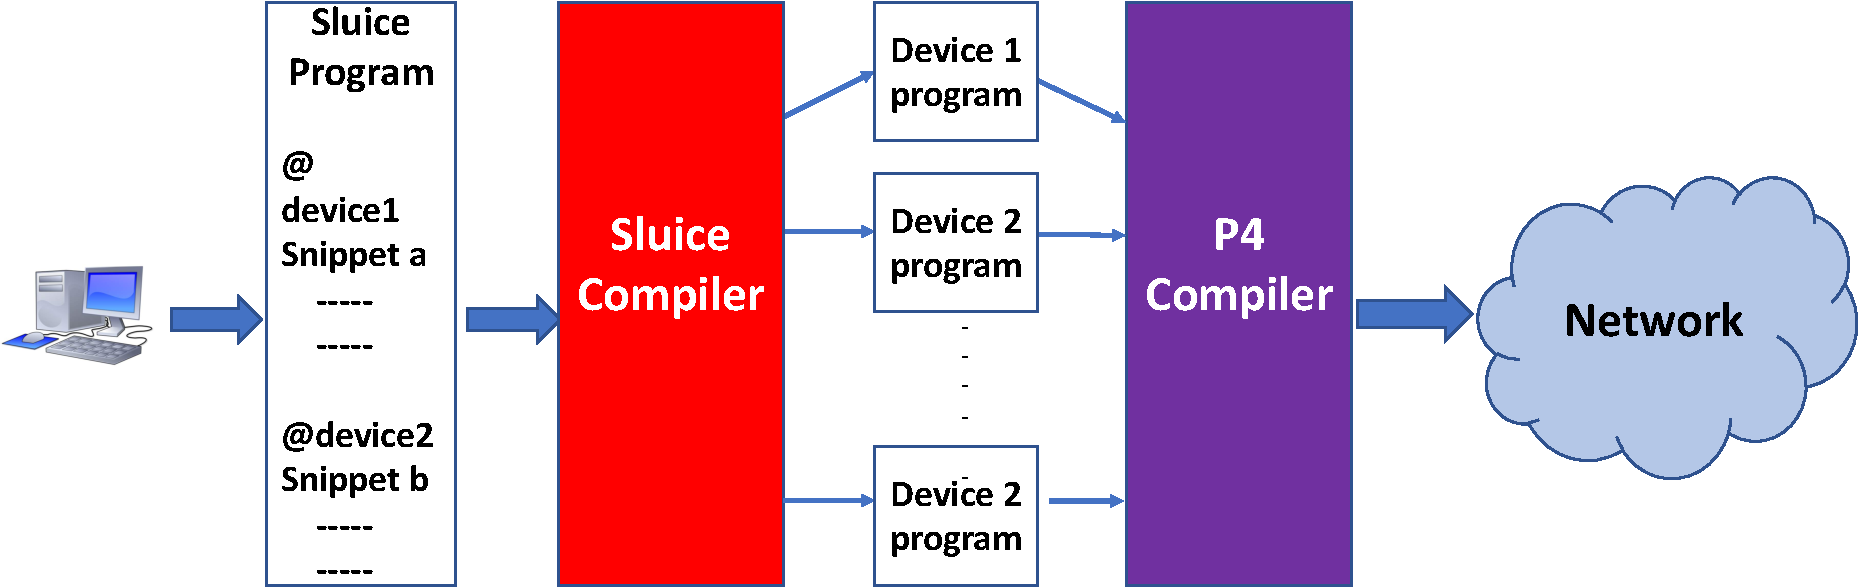
\includegraphics[width=90mm,scale=0.7]{figures/sluice_workflow.pdf}
\caption{Sluice Workflow}
\vspace{-7mm}
\end{figure}
\vspace{-3mm}

\section{Sluice Design}
In the Sluice model, a network-wide program consists of high-level code
\textit{snippets} annotated by the operator to run on particular devices in a
network. The code in each snippet is to be executed on packets arriving at its
corresponding device. Snippets support a variety of operations:
read-from/write-to packets; arithmetic using packet data, local variables, or
stateful register arrays; and control flow statements. To handle computation on
custom packet headers not supported by default (eth/ip/tcp/udp), users may
define packet header declarations similar to C structs. An optional annotation
in the declaration, the parser condition, automatically generates a header
parser for these user-defined headers. Sluice programs may also import
device-specific variables/attributes for use in code snippets. Sluice also lets
the programmer restrict snippets to operate on specific flows or IP address
ranges.

Figure 1 describes the Sluice workflow. The compiler translates each snippet of
a sluice program into a device-specific program. After initial parsing, lines
of code in the snippet are decomposed into a directed acyclic graph (DAG) that
maps dependencies between variables in each snippet. This graph is then passed
to the backend of the compiler that generates the corresponding P4 program for
that device, for example bmv2 or Tofino.\footnote{Currently we only support
bmv2 but plan to support more devices.} 

%Example of citation here\cite{floyd1993random, stoica2001chord}

\section{Demonstrations}
 
\subsection{Traffic Matrix}

Figure 2 displays the Mininet network topology for our traffic matrix demo.
Packets are sent over UDP from each host to all other hosts according to a
Poisson traffic model with mean inter-arrival time of 0.5 seconds. The codelet
below is our Sluice program with a single snippet \textit{traffic\_example}
that is launched on all switches of the network. To run the simulation, the
user passes the Sluice program and network topology to the compiler. The
compiler generates P4 code to run on each switch as well as control plane table
entries for routing packets through the topology.

\begin{lstlisting}[language=Python, basicstyle=\scriptsize]
import device psa;

packet p: udp(srcPort:1234)
  nhops : bit<32>;

@ bmv2 : ;
snippet traffic_example()
  persistent cnt : bit<32>[10];
  cnt[psa.ingress_port] = cnt[psa.ingress_port] + 1;
  p.nhops = p.nhops + 1;
\end{lstlisting}

This demo shows how a simple Sluice program can be used to enable each switch
to measure link usage for a specific flow of user-defined packets on UDP
srcPort 1234. Each packet \textit{p} contains a custom header \textit{nhops}
that is incremented each time the packet enters a switch to inform the
receiving host of the number of hops the packet took. Each switch maintains a
stateful register counter \textit{cnt}, indexed by switch ingress port, that
tracks how many packets have entered through that ingress port. Aggregated over
all switches, these counters represent a matrix measuring each link's
usage in the network at a given time. This matrix (residing on the whole
network) is then queried once every second from the control plane to generate
time-series plots of link-utilization for each link. Figure 3 displays the
histogram of packet rates on link s1-s3 after collecting data for 15 minutes.
The expected distribution of packet rates \textit{Poisson}($\mu = 2$
packets/sec) is also plotted to confirm the accuracy of the Mininet emulation.

\begin{figure}[tp]
\centering
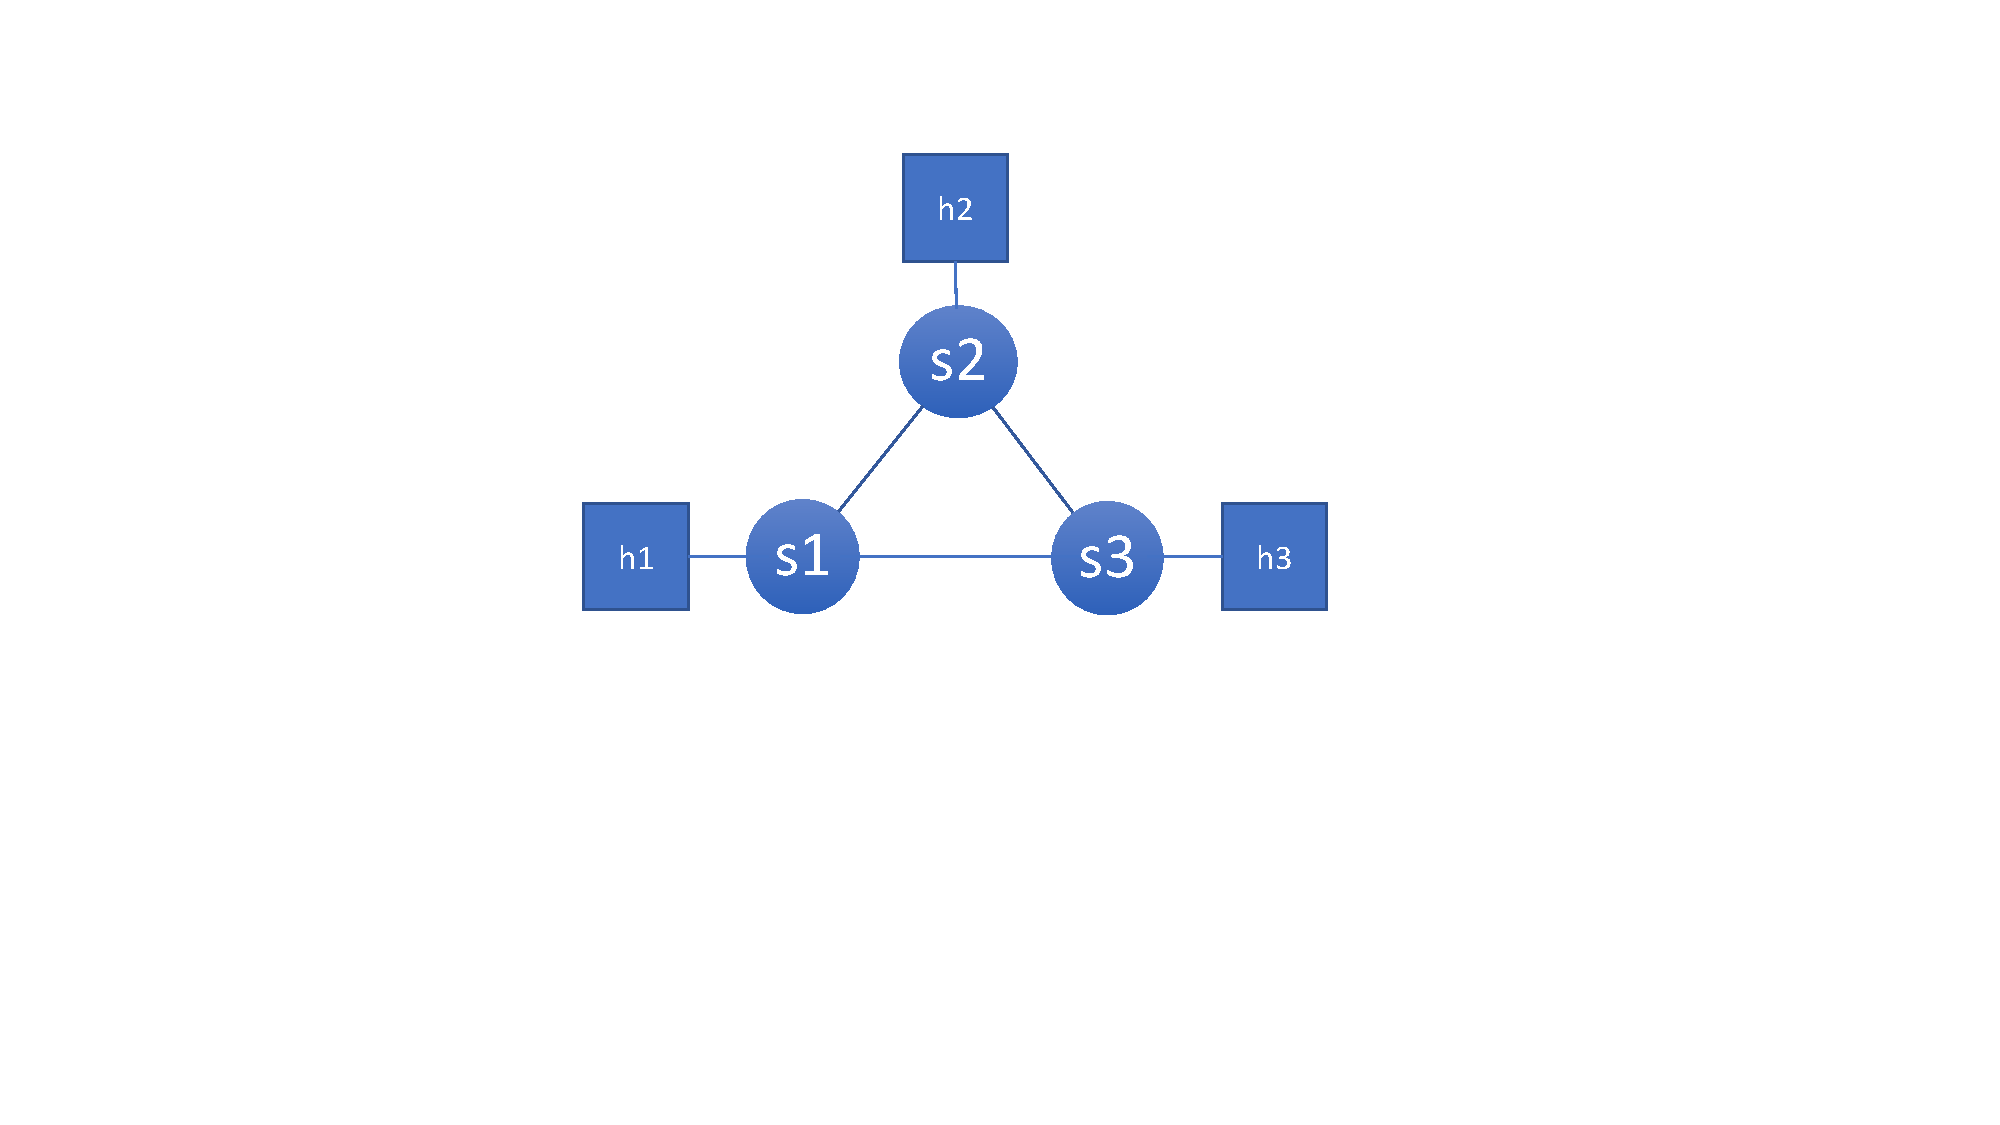
\includegraphics[width=40mm,scale=0.7]{figures/traf_mat_topo}
\caption{Topology For Traffic Matrix Demo}
\end{figure}

 \vspace{-4mm}

\begin{figure}[tp]
\centering
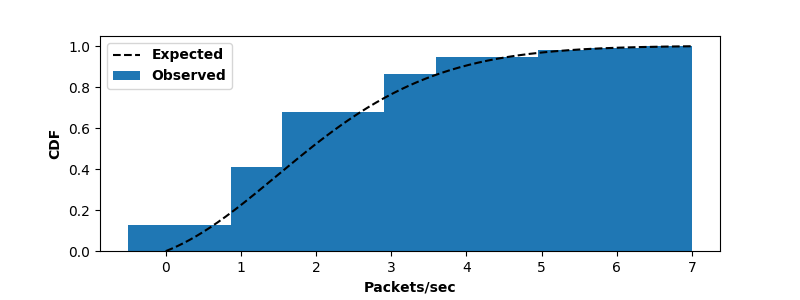
\includegraphics[width=90mm,scale=0.7]{figures/exp_obs_cdf}
\caption{CDF of Packet Rate on link s1-s3}
\end{figure}

 \vspace{1mm}
\subsection{Stream processing}
 \vspace{-1mm}

This example demonstrates a simple join-filter operation between two streams of
tuples. A stream is an unbounded table where a packet represents a tuple of
data (\textit{ad\_id, impression\_time, click\_time}) enclosed in a custom
header. The topology in Figure 4 describes the data flow and shows how an
operator query runs on the switches of the network. Host 1 sends a stream of ad
impressions while Host 2 sends a stream of ad clicks. The two streams are
joined on the \textit{ad\_id} field at s1 and filtered on the \textit{ad\_id}
field at s2 and the result is sent to h3. 

\begin{figure}[tp]
\centering
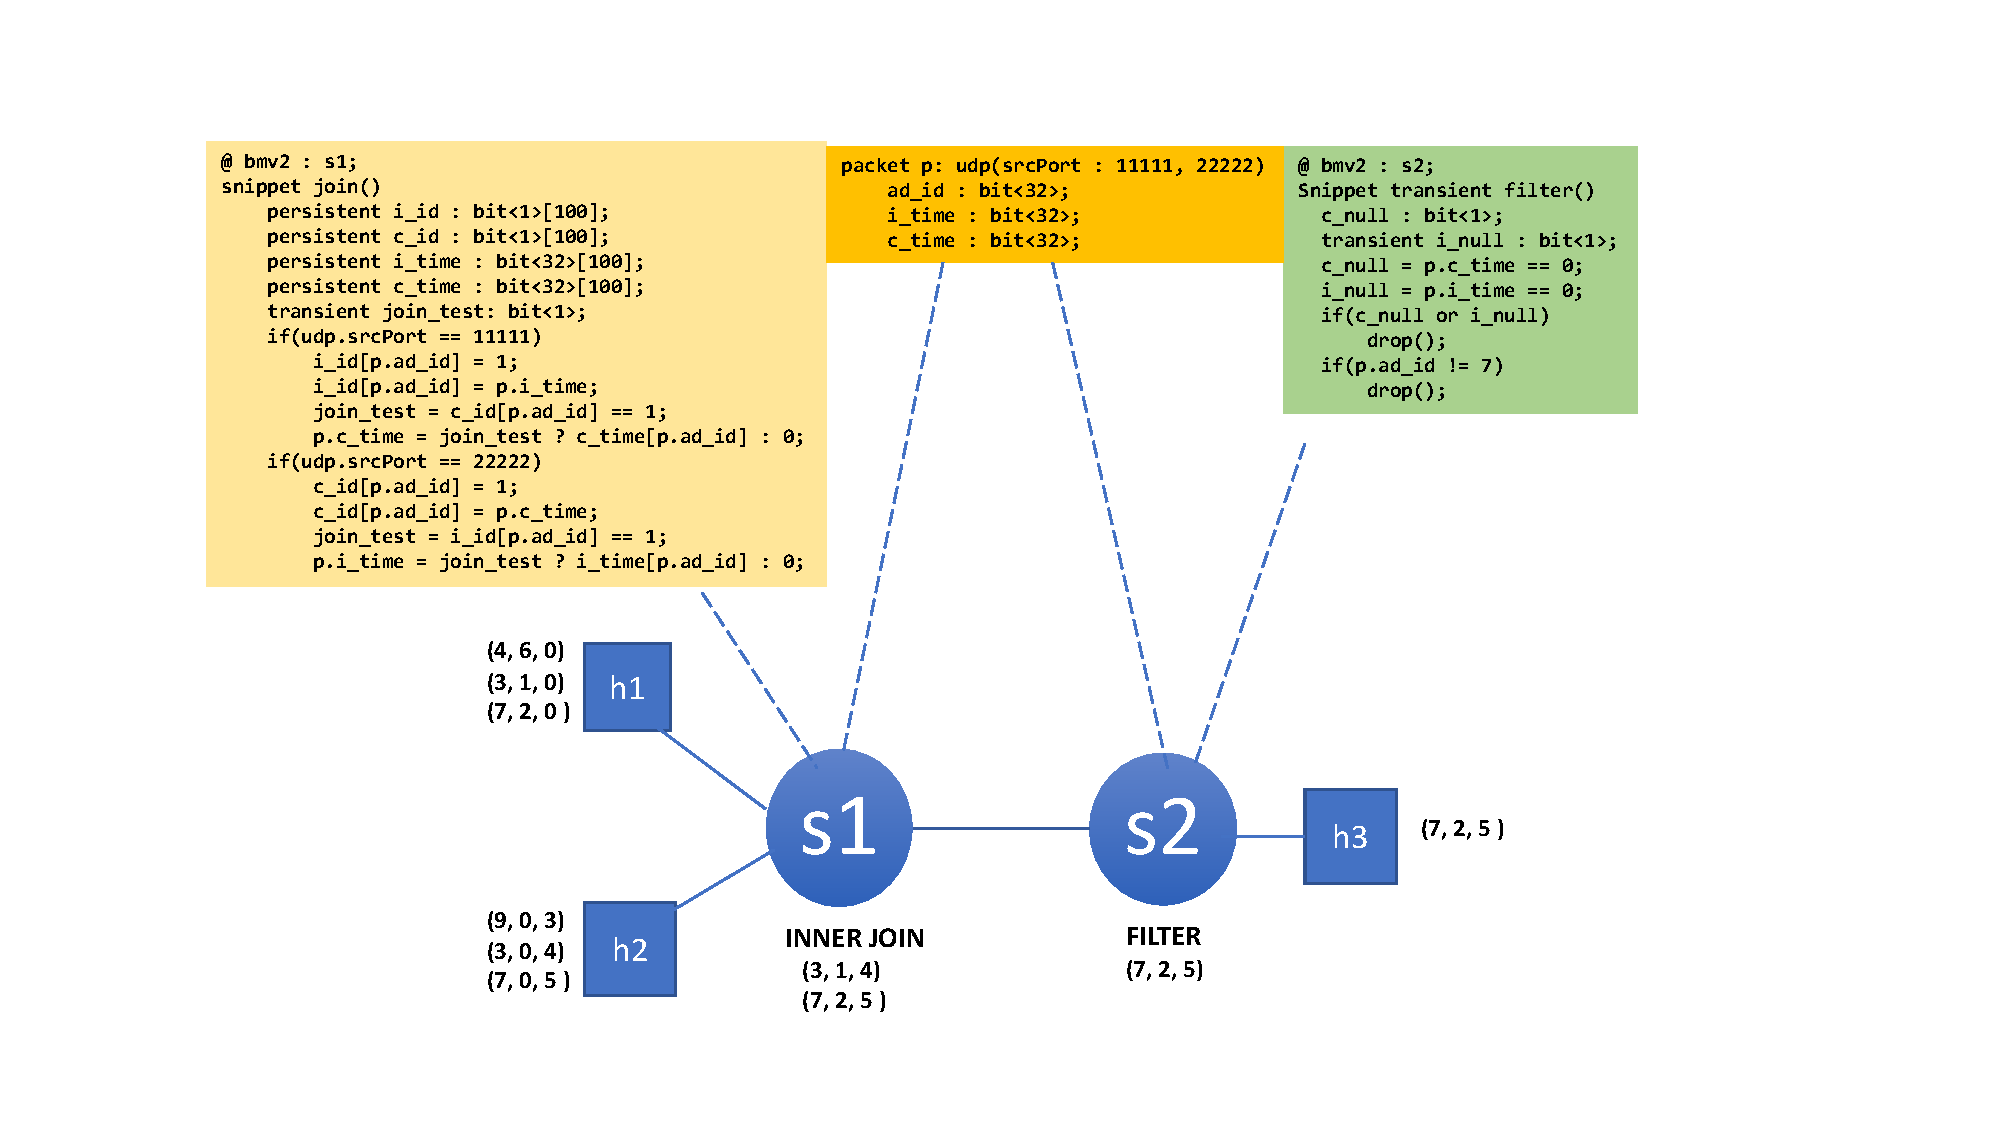
\includegraphics[width=88mm]{figures/streaming_example}
\caption{Streaming example topology, data flow, and code placement on switches}
\vspace{-5mm}
\end{figure}
\vspace{-3mm}


%\section{Future Work}
%\textbf{An optimizing Sluice compiler.} We envision using the dependency DAG to
%provide several automatic optimizations or code transformations. For example,
%it is possible that certain lines of code in a snippet cannot be run on the
%device annotated by the operator, e.g., programmable switching chips have
%limited support for floating point or complex string operations. Code
%containing such features must be moved to the control plane or an end host data
%plane while at the same time, preserving the original program semantics
%intended by the operator. Doing this automatically would free the Sluice
%programmer from reasoning about these semantics.
%%
%%\textbf{Supporting multi-tenancy.} Another area of future work is allowing
%%Sluice \rn{would this really be a change to Sluice? Or would this be using
%%Sluice to do something else?} to support multiple tenants with their own Sluice
%%programs running on their own virtual networks overlayed on the same physical
%%topology. If each tenant wants to run their own network-wide program on their
%%virtual topology, the network operator will need to merge all these into one
%%data plane implementation that runs on the entire physical network. Extending
%%Sluice to support this multi-tenancy use case would allow us to provide the
%%same benefits to the data plane that multi-tenant network
%%virtualization~\cite{nvp} provided for the control plane.




